\documentclass[twoside]{book}

% Packages required by doxygen
\usepackage{fixltx2e}
\usepackage{calc}
\usepackage{doxygen}
\usepackage[export]{adjustbox} % also loads graphicx
\usepackage{graphicx}
\usepackage[utf8]{inputenc}
\usepackage{makeidx}
\usepackage{multicol}
\usepackage{multirow}
\PassOptionsToPackage{warn}{textcomp}
\usepackage{textcomp}
\usepackage[nointegrals]{wasysym}
\usepackage[table]{xcolor}

% Font selection
\usepackage[T1]{fontenc}
\usepackage[scaled=.90]{helvet}
\usepackage{courier}
\usepackage{amssymb}
\usepackage{sectsty}
\renewcommand{\familydefault}{\sfdefault}
\allsectionsfont{%
  \fontseries{bc}\selectfont%
  \color{darkgray}%
}
\renewcommand{\DoxyLabelFont}{%
  \fontseries{bc}\selectfont%
  \color{darkgray}%
}
\newcommand{\+}{\discretionary{\mbox{\scriptsize$\hookleftarrow$}}{}{}}

% Page & text layout
\usepackage{geometry}
\geometry{%
  a4paper,%
  top=2.5cm,%
  bottom=2.5cm,%
  left=2.5cm,%
  right=2.5cm%
}
\tolerance=750
\hfuzz=15pt
\hbadness=750
\setlength{\emergencystretch}{15pt}
\setlength{\parindent}{0cm}
\setlength{\parskip}{3ex plus 2ex minus 2ex}
\makeatletter
\renewcommand{\paragraph}{%
  \@startsection{paragraph}{4}{0ex}{-1.0ex}{1.0ex}{%
    \normalfont\normalsize\bfseries\SS@parafont%
  }%
}
\renewcommand{\subparagraph}{%
  \@startsection{subparagraph}{5}{0ex}{-1.0ex}{1.0ex}{%
    \normalfont\normalsize\bfseries\SS@subparafont%
  }%
}
\makeatother

% Headers & footers
\usepackage{fancyhdr}
\pagestyle{fancyplain}
\fancyhead[LE]{\fancyplain{}{\bfseries\thepage}}
\fancyhead[CE]{\fancyplain{}{}}
\fancyhead[RE]{\fancyplain{}{\bfseries\leftmark}}
\fancyhead[LO]{\fancyplain{}{\bfseries\rightmark}}
\fancyhead[CO]{\fancyplain{}{}}
\fancyhead[RO]{\fancyplain{}{\bfseries\thepage}}
\fancyfoot[LE]{\fancyplain{}{}}
\fancyfoot[CE]{\fancyplain{}{}}
\fancyfoot[RE]{\fancyplain{}{\bfseries\scriptsize Generated by Doxygen }}
\fancyfoot[LO]{\fancyplain{}{\bfseries\scriptsize Generated by Doxygen }}
\fancyfoot[CO]{\fancyplain{}{}}
\fancyfoot[RO]{\fancyplain{}{}}
\renewcommand{\footrulewidth}{0.4pt}
\renewcommand{\chaptermark}[1]{%
  \markboth{#1}{}%
}
\renewcommand{\sectionmark}[1]{%
  \markright{\thesection\ #1}%
}

% Indices & bibliography
\usepackage{natbib}
\usepackage[titles]{tocloft}
\setcounter{tocdepth}{3}
\setcounter{secnumdepth}{5}
\makeindex

% Hyperlinks (required, but should be loaded last)
\usepackage{ifpdf}
\ifpdf
  \usepackage[pdftex,pagebackref=true]{hyperref}
\else
  \usepackage[ps2pdf,pagebackref=true]{hyperref}
\fi
\hypersetup{%
  colorlinks=true,%
  linkcolor=blue,%
  citecolor=blue,%
  unicode%
}

% Custom commands
\newcommand{\clearemptydoublepage}{%
  \newpage{\pagestyle{empty}\cleardoublepage}%
}

\usepackage{caption}
\captionsetup{labelsep=space,justification=centering,font={bf},singlelinecheck=off,skip=4pt,position=top}

%===== C O N T E N T S =====

\begin{document}

% Titlepage & ToC
\hypersetup{pageanchor=false,
             bookmarksnumbered=true,
             pdfencoding=unicode
            }
\pagenumbering{alph}
\begin{titlepage}
\vspace*{7cm}
\begin{center}%
{\Large Multiple Shooting \\[1ex]\large 1 }\\
\vspace*{1cm}
{\large Generated by Doxygen 1.8.13}\\
\end{center}
\end{titlepage}
\clearemptydoublepage
\pagenumbering{roman}
\tableofcontents
\clearemptydoublepage
\pagenumbering{arabic}
\hypersetup{pageanchor=true}

%--- Begin generated contents ---
\chapter{Hierarchical Index}
\section{Class Hierarchy}
This inheritance list is sorted roughly, but not completely, alphabetically\+:\begin{DoxyCompactList}
\item \contentsline{section}{Boundary\+Condition}{\pageref{classBoundaryCondition}}{}
\begin{DoxyCompactList}
\item \contentsline{section}{B\+C\+\_\+\+Linear}{\pageref{classBC__Linear}}{}
\end{DoxyCompactList}
\item \contentsline{section}{Curve}{\pageref{classCurve}}{}
\begin{DoxyCompactList}
\item \contentsline{section}{Curve\+TF}{\pageref{classCurveTF}}{}
\item \contentsline{section}{Test\+:\+:Curve\+Stoer}{\pageref{classTest_1_1CurveStoer}}{}
\item \contentsline{section}{Test\+:\+:Curve\+Troesch}{\pageref{classTest_1_1CurveTroesch}}{}
\end{DoxyCompactList}
\item \contentsline{section}{D\+O\+P\+R\+I54}{\pageref{structDOPRI54}}{}
\item \contentsline{section}{D\+O\+P\+R\+I87}{\pageref{structDOPRI87}}{}
\item \contentsline{section}{E\+R\+K\+\_\+04}{\pageref{structERK__04}}{}
\item \contentsline{section}{F\+A\+D\+\_\+\+Setup$<$ Callable $>$}{\pageref{classFAD__Setup}}{}
\item \contentsline{section}{Functor}{\pageref{classFunctor}}{}
\begin{DoxyCompactList}
\item \contentsline{section}{Div\+Functor}{\pageref{classDivFunctor}}{}
\begin{DoxyCompactList}
\item \contentsline{section}{F\+A\+D\+\_\+c\+Wrapper$<$ Callable $>$}{\pageref{classFAD__cWrapper}}{}
\item \contentsline{section}{Multiple\+Shooting}{\pageref{classMultipleShooting}}{}
\item \contentsline{section}{Single\+Shooting}{\pageref{classSingleShooting}}{}
\end{DoxyCompactList}
\item \contentsline{section}{std\+\_\+c\+Wrapper$<$ Callable $>$}{\pageref{classstd__cWrapper}}{}
\end{DoxyCompactList}
\item \contentsline{section}{Gnu\+Plot}{\pageref{classGnuPlot}}{}
\item \contentsline{section}{K\+A\+RP}{\pageref{structKARP}}{}
\item \contentsline{section}{Newton$<$ Callable $>$}{\pageref{classNewton}}{}
\item \contentsline{section}{One\+Step\+Method}{\pageref{classOneStepMethod}}{}
\begin{DoxyCompactList}
\item \contentsline{section}{Blackbox}{\pageref{classBlackbox}}{}
\item \contentsline{section}{E\+RK$<$ Butcher\+Tableau $>$}{\pageref{classERK}}{}
\item \contentsline{section}{E\+R\+K\+\_\+\+Test\+\_\+04}{\pageref{classERK__Test__04}}{}
\item \contentsline{section}{Euler}{\pageref{classEuler}}{}
\end{DoxyCompactList}
\item \contentsline{section}{R\+K65}{\pageref{structRK65}}{}
\item \contentsline{section}{Shooting\+Function}{\pageref{classShootingFunction}}{}
\begin{DoxyCompactList}
\item \contentsline{section}{S\+F\+\_\+\+Automatic$<$ M, M\+\_\+\+Var $>$}{\pageref{classSF__Automatic}}{}
\item \contentsline{section}{S\+F\+\_\+\+External$<$ M $>$}{\pageref{classSF__External}}{}
\end{DoxyCompactList}
\item \contentsline{section}{Time\+Functor}{\pageref{classTimeFunctor}}{}
\begin{DoxyCompactList}
\item \contentsline{section}{std\+\_\+t\+Wrapper$<$ Callable $>$}{\pageref{classstd__tWrapper}}{}
\item \contentsline{section}{Time\+Div\+Functor}{\pageref{classTimeDivFunctor}}{}
\begin{DoxyCompactList}
\item \contentsline{section}{F\+A\+D\+\_\+t\+Wrapper$<$ Callable $>$}{\pageref{classFAD__tWrapper}}{}
\end{DoxyCompactList}
\end{DoxyCompactList}
\end{DoxyCompactList}

\chapter{Class Index}
\section{Class List}
Here are the classes, structs, unions and interfaces with brief descriptions\+:\begin{DoxyCompactList}
\item\contentsline{section}{\hyperlink{classBC__Linear}{B\+C\+\_\+\+Linear} }{\pageref{classBC__Linear}}{}
\item\contentsline{section}{\hyperlink{classBlackbox}{Blackbox} }{\pageref{classBlackbox}}{}
\item\contentsline{section}{\hyperlink{classBoundaryCondition}{Boundary\+Condition} }{\pageref{classBoundaryCondition}}{}
\item\contentsline{section}{\hyperlink{classCurve}{Curve} }{\pageref{classCurve}}{}
\item\contentsline{section}{\hyperlink{classTest_1_1CurveStoer}{Test\+::\+Curve\+Stoer} }{\pageref{classTest_1_1CurveStoer}}{}
\item\contentsline{section}{\hyperlink{classCurveTF}{Curve\+TF} }{\pageref{classCurveTF}}{}
\item\contentsline{section}{\hyperlink{classTest_1_1CurveTroesch}{Test\+::\+Curve\+Troesch} }{\pageref{classTest_1_1CurveTroesch}}{}
\item\contentsline{section}{\hyperlink{classDivFunctor}{Div\+Functor} }{\pageref{classDivFunctor}}{}
\item\contentsline{section}{\hyperlink{structDOPRI}{D\+O\+P\+RI} }{\pageref{structDOPRI}}{}
\item\contentsline{section}{\hyperlink{structDOPRI87}{D\+O\+P\+R\+I87} }{\pageref{structDOPRI87}}{}
\item\contentsline{section}{\hyperlink{classERK}{E\+R\+K$<$ Butcher\+Tableau $>$} }{\pageref{classERK}}{}
\item\contentsline{section}{\hyperlink{structERK__04}{E\+R\+K\+\_\+04} }{\pageref{structERK__04}}{}
\item\contentsline{section}{\hyperlink{classERK__Test__04}{E\+R\+K\+\_\+\+Test\+\_\+04} }{\pageref{classERK__Test__04}}{}
\item\contentsline{section}{\hyperlink{classEuler}{Euler} }{\pageref{classEuler}}{}
\item\contentsline{section}{\hyperlink{classFAD__cWrapper}{F\+A\+D\+\_\+c\+Wrapper$<$ Callable $>$} }{\pageref{classFAD__cWrapper}}{}
\item\contentsline{section}{\hyperlink{classFAD__Setup}{F\+A\+D\+\_\+\+Setup$<$ Callable $>$} }{\pageref{classFAD__Setup}}{}
\item\contentsline{section}{\hyperlink{classFAD__tWrapper}{F\+A\+D\+\_\+t\+Wrapper$<$ Callable $>$} }{\pageref{classFAD__tWrapper}}{}
\item\contentsline{section}{\hyperlink{classFunctor}{Functor} }{\pageref{classFunctor}}{}
\item\contentsline{section}{\hyperlink{classGnuPlot}{Gnu\+Plot} }{\pageref{classGnuPlot}}{}
\item\contentsline{section}{\hyperlink{structKARP}{K\+A\+RP} }{\pageref{structKARP}}{}
\item\contentsline{section}{\hyperlink{classMultipleShooting}{Multiple\+Shooting$<$ Diff\+Method $>$} }{\pageref{classMultipleShooting}}{}
\item\contentsline{section}{\hyperlink{classNewton}{Newton$<$ Callable $>$} }{\pageref{classNewton}}{}
\item\contentsline{section}{\hyperlink{classOneStepMethod}{One\+Step\+Method} }{\pageref{classOneStepMethod}}{}
\item\contentsline{section}{\hyperlink{structRK65}{R\+K65} }{\pageref{structRK65}}{}
\item\contentsline{section}{\hyperlink{classSF__Automatic}{S\+F\+\_\+\+Automatic} }{\pageref{classSF__Automatic}}{}
\item\contentsline{section}{\hyperlink{classSF__External}{S\+F\+\_\+\+External} }{\pageref{classSF__External}}{}
\item\contentsline{section}{\hyperlink{classShootingFunction}{Shooting\+Function} }{\pageref{classShootingFunction}}{}
\item\contentsline{section}{\hyperlink{classSingleShooting}{Single\+Shooting$<$ Diff\+Method $>$} }{\pageref{classSingleShooting}}{}
\item\contentsline{section}{\hyperlink{classstd__cWrapper}{std\+\_\+c\+Wrapper$<$ Callable $>$} }{\pageref{classstd__cWrapper}}{}
\item\contentsline{section}{\hyperlink{classstd__tWrapper}{std\+\_\+t\+Wrapper$<$ Callable $>$} }{\pageref{classstd__tWrapper}}{}
\item\contentsline{section}{\hyperlink{classTimeDivFunctor}{Time\+Div\+Functor} }{\pageref{classTimeDivFunctor}}{}
\item\contentsline{section}{\hyperlink{classTimeFunctor}{Time\+Functor} }{\pageref{classTimeFunctor}}{}
\end{DoxyCompactList}

\chapter{Class Documentation}
\hypertarget{classBlackbox}{}\section{Blackbox Class Reference}
\label{classBlackbox}\index{Blackbox@{Blackbox}}


Inheritance diagram for Blackbox\+:
\nopagebreak
\begin{figure}[H]
\begin{center}
\leavevmode
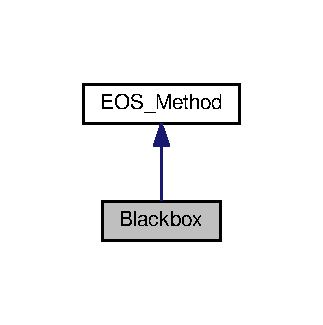
\includegraphics[width=167pt]{classBlackbox__inherit__graph}
\end{center}
\end{figure}


Collaboration diagram for Blackbox\+:
\nopagebreak
\begin{figure}[H]
\begin{center}
\leavevmode
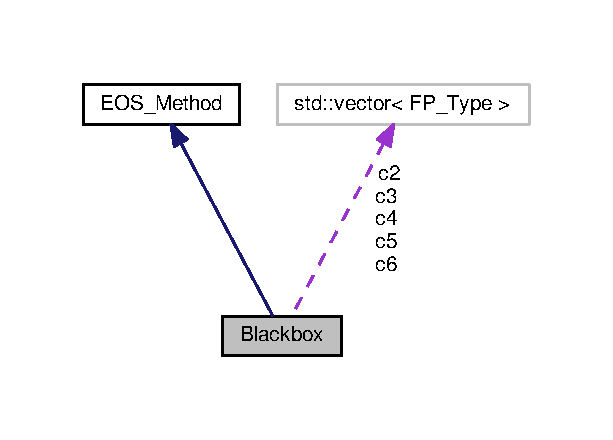
\includegraphics[width=306pt]{classBlackbox__coll__graph}
\end{center}
\end{figure}
\subsection*{Public Member Functions}
\begin{DoxyCompactItemize}
\item 
\mbox{\Hypertarget{classBlackbox_a38b421a2cc7fa40d8dadf09f44b9b80a}\label{classBlackbox_a38b421a2cc7fa40d8dadf09f44b9b80a}} 
virtual dealii\+::\+Vector$<$ F\+P\+\_\+\+Type $>$ {\bfseries increment\+\_\+function} (const F\+P\+\_\+\+Type t, const dealii\+::\+Vector$<$ F\+P\+\_\+\+Type $>$ \&y, const F\+P\+\_\+\+Type h) override
\end{DoxyCompactItemize}
\subsection*{Public Attributes}
\begin{DoxyCompactItemize}
\item 
\mbox{\Hypertarget{classBlackbox_a0a9ceb8a67769f231b2c958fd1205042}\label{classBlackbox_a0a9ceb8a67769f231b2c958fd1205042}} 
const std\+::vector$<$ F\+P\+\_\+\+Type $>$ {\bfseries c2} = \{ 1./5, 1./5 \}
\item 
\mbox{\Hypertarget{classBlackbox_ac1b78c2e2779213a170e072a41de9221}\label{classBlackbox_ac1b78c2e2779213a170e072a41de9221}} 
const std\+::vector$<$ F\+P\+\_\+\+Type $>$ {\bfseries c3} = \{ 3./10, 3./40, 9./40 \}
\item 
\mbox{\Hypertarget{classBlackbox_a2064bec0552fd00792c4da06e58fbae6}\label{classBlackbox_a2064bec0552fd00792c4da06e58fbae6}} 
const std\+::vector$<$ F\+P\+\_\+\+Type $>$ {\bfseries c4} = \{ 4./5, 44./45, 56./15, 32./9 \}
\item 
const std\+::vector$<$ F\+P\+\_\+\+Type $>$ {\bfseries c5}
\item 
const std\+::vector$<$ F\+P\+\_\+\+Type $>$ {\bfseries c6}
\item 
\mbox{\Hypertarget{classBlackbox_ae46f4feda59f07bf81903aeac86c676e}\label{classBlackbox_ae46f4feda59f07bf81903aeac86c676e}} 
const F\+P\+\_\+\+Type {\bfseries s1} = 35./384
\item 
\mbox{\Hypertarget{classBlackbox_a3aa11889d818436218abae74cf49db4b}\label{classBlackbox_a3aa11889d818436218abae74cf49db4b}} 
const F\+P\+\_\+\+Type {\bfseries s2} = 0.
\item 
\mbox{\Hypertarget{classBlackbox_ab8a7838aef85aa6c0887a38dbee9fce0}\label{classBlackbox_ab8a7838aef85aa6c0887a38dbee9fce0}} 
const F\+P\+\_\+\+Type {\bfseries s3} = 500./1113
\item 
\mbox{\Hypertarget{classBlackbox_ada127477d1f1d03dd6a7fd543f732c22}\label{classBlackbox_ada127477d1f1d03dd6a7fd543f732c22}} 
const F\+P\+\_\+\+Type {\bfseries s4} = 125./192
\item 
\mbox{\Hypertarget{classBlackbox_a45e3904b06f05528997a4af65e2ea48a}\label{classBlackbox_a45e3904b06f05528997a4af65e2ea48a}} 
const F\+P\+\_\+\+Type {\bfseries s5} = 2187./6784
\item 
\mbox{\Hypertarget{classBlackbox_a5ad4004f7c0f525752bb852f60200f75}\label{classBlackbox_a5ad4004f7c0f525752bb852f60200f75}} 
const F\+P\+\_\+\+Type {\bfseries s6} = 11./84
\end{DoxyCompactItemize}


\subsection{Member Data Documentation}
\mbox{\Hypertarget{classBlackbox_a1bb02f77d852c89644c3b21b0c5f528a}\label{classBlackbox_a1bb02f77d852c89644c3b21b0c5f528a}} 
\index{Blackbox@{Blackbox}!c5@{c5}}
\index{c5@{c5}!Blackbox@{Blackbox}}
\subsubsection{\texorpdfstring{c5}{c5}}
{\footnotesize\ttfamily const std\+::vector$<$F\+P\+\_\+\+Type$>$ Blackbox\+::c5}

{\bfseries Initial value\+:}
\begin{DoxyCode}
= \{ 8./9, 19372./6561, 25360./2187,
                                    64448./6561, 212./729 \}
\end{DoxyCode}
\mbox{\Hypertarget{classBlackbox_aabd96578c54a99b68683fd0114ed5610}\label{classBlackbox_aabd96578c54a99b68683fd0114ed5610}} 
\index{Blackbox@{Blackbox}!c6@{c6}}
\index{c6@{c6}!Blackbox@{Blackbox}}
\subsubsection{\texorpdfstring{c6}{c6}}
{\footnotesize\ttfamily const std\+::vector$<$F\+P\+\_\+\+Type$>$ Blackbox\+::c6}

{\bfseries Initial value\+:}
\begin{DoxyCode}
= \{ 1., 9017./3168, 355./33,
                                    46732./5247, 49./176, 5103./18656 \}
\end{DoxyCode}


The documentation for this class was generated from the following file\+:\begin{DoxyCompactItemize}
\item 
test/test\+\_\+runge\+\_\+kutta.\+h\end{DoxyCompactItemize}

\hypertarget{classDivFunctor}{}\section{Div\+Functor Class Reference}
\label{classDivFunctor}\index{Div\+Functor@{Div\+Functor}}


Inheritance diagram for Div\+Functor\+:
\nopagebreak
\begin{figure}[H]
\begin{center}
\leavevmode
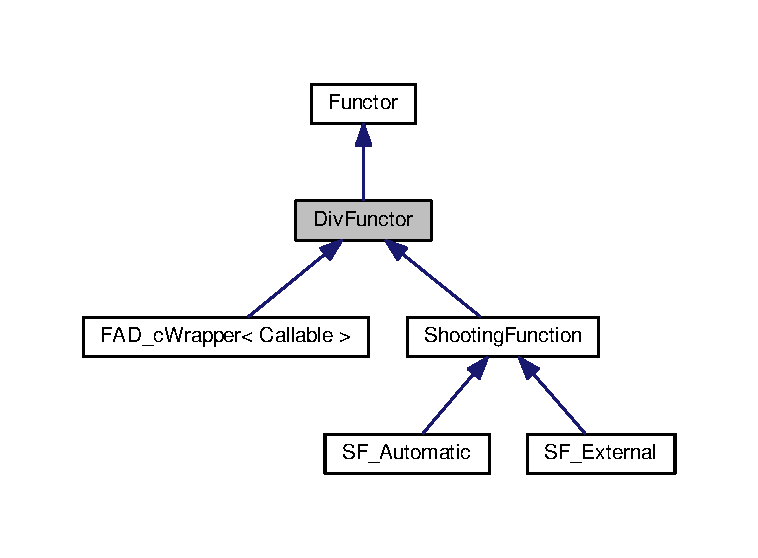
\includegraphics[width=350pt]{classDivFunctor__inherit__graph}
\end{center}
\end{figure}


Collaboration diagram for Div\+Functor\+:
\nopagebreak
\begin{figure}[H]
\begin{center}
\leavevmode
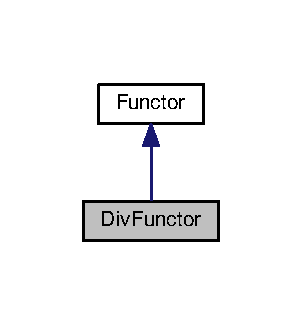
\includegraphics[width=145pt]{classDivFunctor__coll__graph}
\end{center}
\end{figure}
\subsection*{Public Member Functions}
\begin{DoxyCompactItemize}
\item 
\mbox{\Hypertarget{classDivFunctor_aef605410aadd00d345287a539bc81c08}\label{classDivFunctor_aef605410aadd00d345287a539bc81c08}} 
virtual Matrix\+D2 {\bfseries diff} (const Vector\+D2 \&x)=0
\end{DoxyCompactItemize}


The documentation for this class was generated from the following file\+:\begin{DoxyCompactItemize}
\item 
lac/lac\+\_\+types.\+h\end{DoxyCompactItemize}

\hypertarget{structDOPRI}{}\section{D\+O\+P\+RI Struct Reference}
\label{structDOPRI}\index{D\+O\+P\+RI@{D\+O\+P\+RI}}


Collaboration diagram for D\+O\+P\+RI\+:\nopagebreak
\begin{figure}[H]
\begin{center}
\leavevmode
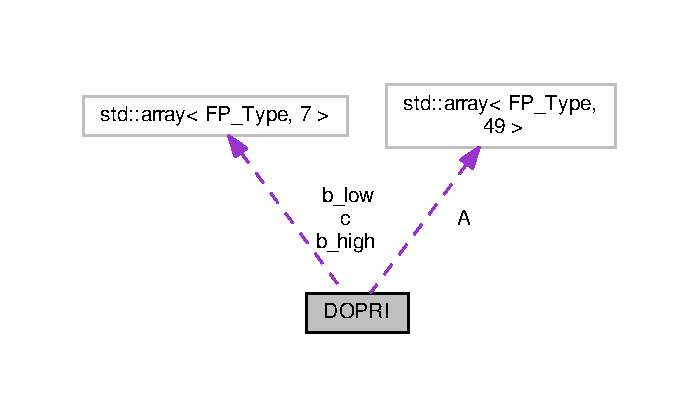
\includegraphics[width=336pt]{structDOPRI__coll__graph}
\end{center}
\end{figure}
\subsection*{Public Attributes}
\begin{DoxyCompactItemize}
\item 
\mbox{\Hypertarget{structDOPRI_a3520af988d456d6f669ba92fae81cea2}\label{structDOPRI_a3520af988d456d6f669ba92fae81cea2}} 
const size\+\_\+t {\bfseries n} = 7
\item 
const std\+::array$<$ F\+P\+\_\+\+Type, 7 $>$ {\bfseries c}
\item 
const std\+::array$<$ F\+P\+\_\+\+Type, 49 $>$ {\bfseries A}
\item 
const std\+::array$<$ F\+P\+\_\+\+Type, 7 $>$ {\bfseries b\+\_\+high}
\item 
const std\+::array$<$ F\+P\+\_\+\+Type, 7 $>$ {\bfseries b\+\_\+low}
\end{DoxyCompactItemize}


\subsection{Member Data Documentation}
\mbox{\Hypertarget{structDOPRI_a65a11509e008348c328fa217fc7538a2}\label{structDOPRI_a65a11509e008348c328fa217fc7538a2}} 
\index{D\+O\+P\+RI@{D\+O\+P\+RI}!A@{A}}
\index{A@{A}!D\+O\+P\+RI@{D\+O\+P\+RI}}
\subsubsection{\texorpdfstring{A}{A}}
{\footnotesize\ttfamily const std\+::array$<$F\+P\+\_\+\+Type, 49$>$ D\+O\+P\+R\+I\+::A}

{\bfseries Initial value\+:}
\begin{DoxyCode}
= \{
    0,            0,             0,            0,          0,             0,       0,
    1./5,         0,             0,            0,          0,             0,       0,
    3./40,        9./40,         0,            0,          0,             0,       0,
    44./45,       -56./15,       32./9,        0,          0,             0,       0,
    19372./6561,  -25360./2187,  64448./6561,  -212./729,  0,             0,       0,
    9017./3168,   -355./33,      46732./5247,  49./176,    -5103./18656,  0,       0,
    35./384,      0,             500./1113,    125./192,   -2187./6784,   11./84,  0
  \}
\end{DoxyCode}
\mbox{\Hypertarget{structDOPRI_ac3af90d1e84f3d0ec14ed0247afff8f6}\label{structDOPRI_ac3af90d1e84f3d0ec14ed0247afff8f6}} 
\index{D\+O\+P\+RI@{D\+O\+P\+RI}!b\+\_\+high@{b\+\_\+high}}
\index{b\+\_\+high@{b\+\_\+high}!D\+O\+P\+RI@{D\+O\+P\+RI}}
\subsubsection{\texorpdfstring{b\+\_\+high}{b\_high}}
{\footnotesize\ttfamily const std\+::array$<$F\+P\+\_\+\+Type, 7$>$ D\+O\+P\+R\+I\+::b\+\_\+high}

{\bfseries Initial value\+:}
\begin{DoxyCode}
= \{
    35./384, 0, 500./1113, 125./192, -2187./6784, 11./84, 0
  \}
\end{DoxyCode}
\mbox{\Hypertarget{structDOPRI_a82910ddf39b454e7fcb2bccb35b064d0}\label{structDOPRI_a82910ddf39b454e7fcb2bccb35b064d0}} 
\index{D\+O\+P\+RI@{D\+O\+P\+RI}!b\+\_\+low@{b\+\_\+low}}
\index{b\+\_\+low@{b\+\_\+low}!D\+O\+P\+RI@{D\+O\+P\+RI}}
\subsubsection{\texorpdfstring{b\+\_\+low}{b\_low}}
{\footnotesize\ttfamily const std\+::array$<$F\+P\+\_\+\+Type, 7$>$ D\+O\+P\+R\+I\+::b\+\_\+low}

{\bfseries Initial value\+:}
\begin{DoxyCode}
= \{
    5179./57600, 0, 7571./16695, 393./640, -92097./339200, 187./2100, 1./40
  \}
\end{DoxyCode}
\mbox{\Hypertarget{structDOPRI_aee5aa453f5692dbb6b39a5575ab7736f}\label{structDOPRI_aee5aa453f5692dbb6b39a5575ab7736f}} 
\index{D\+O\+P\+RI@{D\+O\+P\+RI}!c@{c}}
\index{c@{c}!D\+O\+P\+RI@{D\+O\+P\+RI}}
\subsubsection{\texorpdfstring{c}{c}}
{\footnotesize\ttfamily const std\+::array$<$F\+P\+\_\+\+Type, 7$>$ D\+O\+P\+R\+I\+::c}

{\bfseries Initial value\+:}
\begin{DoxyCode}
= \{
    0, 1./5, 3./10, 4./5, 8./9, 1., 1.
  \}
\end{DoxyCode}


The documentation for this struct was generated from the following file\+:\begin{DoxyCompactItemize}
\item 
ivp/tableau.\+h\end{DoxyCompactItemize}

\hypertarget{structDOPRI87}{}\section{D\+O\+P\+R\+I87 Struct Reference}
\label{structDOPRI87}\index{D\+O\+P\+R\+I87@{D\+O\+P\+R\+I87}}


Collaboration diagram for D\+O\+P\+R\+I87\+:\nopagebreak
\begin{figure}[H]
\begin{center}
\leavevmode
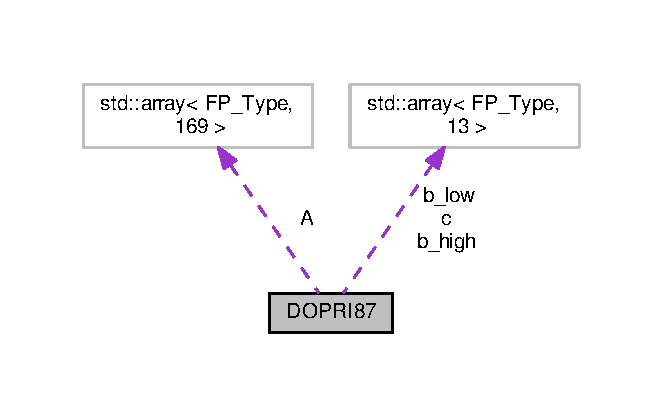
\includegraphics[width=318pt]{structDOPRI87__coll__graph}
\end{center}
\end{figure}
\subsection*{Public Attributes}
\begin{DoxyCompactItemize}
\item 
\mbox{\Hypertarget{structDOPRI87_a5be2549f8041e5c535e477493f284ccb}\label{structDOPRI87_a5be2549f8041e5c535e477493f284ccb}} 
const size\+\_\+t {\bfseries n} = 13
\item 
\mbox{\Hypertarget{structDOPRI87_a765f5d126f15435e636c9f38a554f35f}\label{structDOPRI87_a765f5d126f15435e636c9f38a554f35f}} 
const size\+\_\+t {\bfseries p} = 8
\item 
const std\+::array$<$ F\+P\+\_\+\+Type, 13 $>$ {\bfseries c}
\item 
const std\+::array$<$ F\+P\+\_\+\+Type, 169 $>$ {\bfseries A}
\item 
const std\+::array$<$ F\+P\+\_\+\+Type, 13 $>$ {\bfseries b\+\_\+high}
\item 
const std\+::array$<$ F\+P\+\_\+\+Type, 13 $>$ {\bfseries b\+\_\+low}
\end{DoxyCompactItemize}


\subsection{Member Data Documentation}
\mbox{\Hypertarget{structDOPRI87_a58504e2f3eabbf35b2d4f0e54ebb8d5f}\label{structDOPRI87_a58504e2f3eabbf35b2d4f0e54ebb8d5f}} 
\index{D\+O\+P\+R\+I87@{D\+O\+P\+R\+I87}!A@{A}}
\index{A@{A}!D\+O\+P\+R\+I87@{D\+O\+P\+R\+I87}}
\subsubsection{\texorpdfstring{A}{A}}
{\footnotesize\ttfamily const std\+::array$<$F\+P\+\_\+\+Type, 169$>$ D\+O\+P\+R\+I87\+::A}

{\bfseries Initial value\+:}
\begin{DoxyCode}
= \{
    0,                       0,      0,        0,                          0,                       0,     
                          0,                         0,                         0,                         0,     
                        0,                      0,  0,
    1./18,                   0,      0,        0,                          0,                       0,     
                          0,                         0,                         0,                         0,     
                        0,                      0,  0,
    1./48,                   1./16,  0,        0,                          0,                       0,     
                          0,                         0,                         0,                         0,     
                        0,                      0,  0,
    1./32,                   0,      3./32,    0,                          0,                       0,     
                          0,                         0,                         0,                         0,     
                        0,                      0,  0,
    5./16,                   0,      -75./64,  75./64,                     0,                       0,     
                          0,                         0,                         0,                         0,     
                        0,                      0,  0,
    3./80,                   0,      0,        3./16,                      3./20,                   0,     
                          0,                         0,                         0,                         0,     
                        0,                      0,  0,
    29443841./614563906,     0,      0,        77736538./692538347,        -28693883./1125000000,   
      23124283./1800000000,      0,                         0,                         0,                         0,     
                        0,                      0,  0,
    16016141./946692911,     0,      0,        61564180./158732637,        22789713./633445777,     
      545815736./2771057229,     -180193667./1043307555,    0,                         0,                         0,     
                        0,                      0,  0,
    39632708./573591083,     0,      0,        -433636366./683701615,      -421739975./2616292301,  
      100302831./723423059,      790204164./839813087,      800635310./3783071287,     0,                         0,     
                        0,                      0,  0,
    246121993./1340847787,   0,      0,        -37695042795./15268766246,  -309121744./1061227803,  -
      12992083./490766935,      6005943493./2108947869,    393006217./1396673457,     123872331./1001029789,     0,     
                        0,                      0,  0,
    -1028468189./846180014,  0,      0,        8478235783./508512852,      1311729495./1432422823,  -
      10304129995./1701304382,  -48777925059./3047939560,  15336726248./1032824649,   -45442868181./3398467696,  
      3065993473./597172653,   0,                      0,  0,
    185892177./718116043,    0,      0,        -3185094517./667107341,     -477755414./1098053517,  -
      703635378./230739211,     5731566787./1027545527,    5232866602./850066563,     -4093664535./808688257,    
      3962137247./1805957418,  65686358./487910083,    0,  0,
    403863854./491063109,    0,      0,        -5068492393./434740067,     -411421997./543043805,   
      652783627./914296604,      11173962825./925320556,    -13158990841./6184727034,  3936647629./1978049680,    -
      160528059./685178525,   248638103./1413531060,  0,  0
  \}
\end{DoxyCode}
\mbox{\Hypertarget{structDOPRI87_abd810799ee712d0b3f92bd04474e7fe3}\label{structDOPRI87_abd810799ee712d0b3f92bd04474e7fe3}} 
\index{D\+O\+P\+R\+I87@{D\+O\+P\+R\+I87}!b\+\_\+high@{b\+\_\+high}}
\index{b\+\_\+high@{b\+\_\+high}!D\+O\+P\+R\+I87@{D\+O\+P\+R\+I87}}
\subsubsection{\texorpdfstring{b\+\_\+high}{b\_high}}
{\footnotesize\ttfamily const std\+::array$<$F\+P\+\_\+\+Type, 13$>$ D\+O\+P\+R\+I87\+::b\+\_\+high}

{\bfseries Initial value\+:}
\begin{DoxyCode}
= \{
     14005451./335480064, 0, 0, 0, 0, -59238493./1068277825, 181606767./758867731,   561292985./797845732, 
        -1041891430./1371343529,  760417239./1151165299, 118820643./751138087, -528747749./2220607170,  1./4
   \}
\end{DoxyCode}
\mbox{\Hypertarget{structDOPRI87_a12b1ba26c0d854fdf42760d785bf26d5}\label{structDOPRI87_a12b1ba26c0d854fdf42760d785bf26d5}} 
\index{D\+O\+P\+R\+I87@{D\+O\+P\+R\+I87}!b\+\_\+low@{b\+\_\+low}}
\index{b\+\_\+low@{b\+\_\+low}!D\+O\+P\+R\+I87@{D\+O\+P\+R\+I87}}
\subsubsection{\texorpdfstring{b\+\_\+low}{b\_low}}
{\footnotesize\ttfamily const std\+::array$<$F\+P\+\_\+\+Type, 13$>$ D\+O\+P\+R\+I87\+::b\+\_\+low}

{\bfseries Initial value\+:}
\begin{DoxyCode}
= \{
     13451932./455176623, 0, 0, 0, 0, -808719846./976000145, 1757004468./5645159321, 656045339./265891186, 
        -3867574721./1518517206,   465885868./322736535,  53011238./667516719, 2./45, 0
   \}
\end{DoxyCode}
\mbox{\Hypertarget{structDOPRI87_a4920ff4638ecba0061800d7c456d920d}\label{structDOPRI87_a4920ff4638ecba0061800d7c456d920d}} 
\index{D\+O\+P\+R\+I87@{D\+O\+P\+R\+I87}!c@{c}}
\index{c@{c}!D\+O\+P\+R\+I87@{D\+O\+P\+R\+I87}}
\subsubsection{\texorpdfstring{c}{c}}
{\footnotesize\ttfamily const std\+::array$<$F\+P\+\_\+\+Type, 13$>$ D\+O\+P\+R\+I87\+::c}

{\bfseries Initial value\+:}
\begin{DoxyCode}
= \{
    0., 1./18, 1./12, 1./8, 5./16, 3./8, 59./400, 93./200, 5490023248./9719169821, 13./20, 1201146811./
      1299019798, 1., 1.
  \}
\end{DoxyCode}


The documentation for this struct was generated from the following file\+:\begin{DoxyCompactItemize}
\item 
ivp/tableau.\+h\end{DoxyCompactItemize}

\hypertarget{classEOS__Method}{}\section{E\+O\+S\+\_\+\+Method Class Reference}
\label{classEOS__Method}\index{E\+O\+S\+\_\+\+Method@{E\+O\+S\+\_\+\+Method}}


Inheritance diagram for E\+O\+S\+\_\+\+Method\+:\nopagebreak
\begin{figure}[H]
\begin{center}
\leavevmode
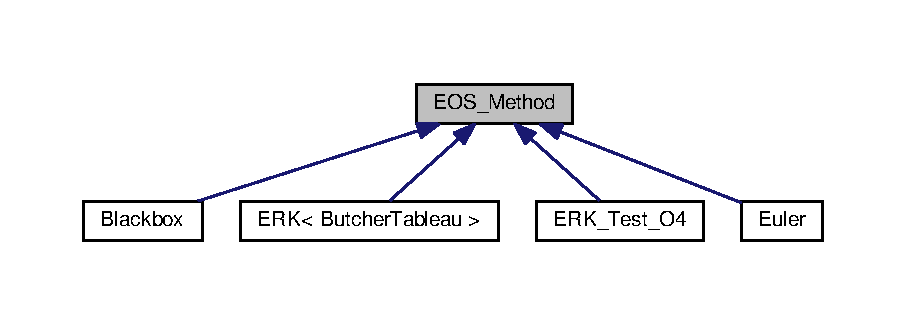
\includegraphics[width=350pt]{classEOS__Method__inherit__graph}
\end{center}
\end{figure}
\subsection*{Public Member Functions}
\begin{DoxyCompactItemize}
\item 
\mbox{\Hypertarget{classEOS__Method_a531d5ee86fcad27fa2299e320417ed26}\label{classEOS__Method_a531d5ee86fcad27fa2299e320417ed26}} 
{\bfseries E\+O\+S\+\_\+\+Method} (\hyperlink{classTimeFunctor}{Time\+Functor} \&\+\_\+f, F\+P\+\_\+\+Type \+\_\+t0, dealii\+::\+Vector$<$ F\+P\+\_\+\+Type $>$ \+\_\+u0)
\item 
\mbox{\Hypertarget{classEOS__Method_a51157a38f285e475337c4e67d1ccd279}\label{classEOS__Method_a51157a38f285e475337c4e67d1ccd279}} 
dealii\+::\+Vector$<$ F\+P\+\_\+\+Type $>$ {\bfseries approx} () const
\item 
\mbox{\Hypertarget{classEOS__Method_a3f7157f6b6518ea3395f90b3c5a795b8}\label{classEOS__Method_a3f7157f6b6518ea3395f90b3c5a795b8}} 
F\+P\+\_\+\+Type {\bfseries endpoint} () const
\item 
\mbox{\Hypertarget{classEOS__Method_aa323926fa9f41a8a011c1a370c2bed7d}\label{classEOS__Method_aa323926fa9f41a8a011c1a370c2bed7d}} 
size\+\_\+t {\bfseries n\+\_\+steps} () const
\item 
\mbox{\Hypertarget{classEOS__Method_ae7f7cd39eddbc7dde0c004773c00ad6e}\label{classEOS__Method_ae7f7cd39eddbc7dde0c004773c00ad6e}} 
void {\bfseries print} (std\+::ostream \&out=std\+::cout) const
\item 
\mbox{\Hypertarget{classEOS__Method_a2abc87316deb095a84ed74e1ddfd56ec}\label{classEOS__Method_a2abc87316deb095a84ed74e1ddfd56ec}} 
void {\bfseries reset} ()
\item 
\mbox{\Hypertarget{classEOS__Method_a8f1d297e535ca2ca7441bafcea43742c}\label{classEOS__Method_a8f1d297e535ca2ca7441bafcea43742c}} 
void {\bfseries save\+\_\+step} (const F\+P\+\_\+\+Type \&t, const dealii\+::\+Vector$<$ F\+P\+\_\+\+Type $>$ \&u)
\item 
\mbox{\Hypertarget{classEOS__Method_a71f54df232ff780bc731b57d24b9f62e}\label{classEOS__Method_a71f54df232ff780bc731b57d24b9f62e}} 
virtual dealii\+::\+Vector$<$ F\+P\+\_\+\+Type $>$ {\bfseries increment\+\_\+function} (F\+P\+\_\+\+Type t, const dealii\+::\+Vector$<$ F\+P\+\_\+\+Type $>$ \&u, F\+P\+\_\+\+Type h)
\item 
\mbox{\Hypertarget{classEOS__Method_a2b2f44ec8d634b8eec6ec51f35425333}\label{classEOS__Method_a2b2f44ec8d634b8eec6ec51f35425333}} 
void {\bfseries iterate\+\_\+up\+\_\+to} (F\+P\+\_\+\+Type t\+\_\+lim, F\+P\+\_\+\+Type h)
\end{DoxyCompactItemize}
\subsection*{Friends}
\begin{DoxyCompactItemize}
\item 
\mbox{\Hypertarget{classEOS__Method_af3aa570b8e278b935d7dc84d2774ccb7}\label{classEOS__Method_af3aa570b8e278b935d7dc84d2774ccb7}} 
class {\bfseries Blackbox}
\item 
\mbox{\Hypertarget{classEOS__Method_a9e8c94ebada889fba517c82fc3408d32}\label{classEOS__Method_a9e8c94ebada889fba517c82fc3408d32}} 
class {\bfseries Euler}
\item 
\mbox{\Hypertarget{classEOS__Method_aaaa2b514e0ee583889d7f78273370f56}\label{classEOS__Method_aaaa2b514e0ee583889d7f78273370f56}} 
class {\bfseries E\+R\+K\+\_\+\+Test\+\_\+\+O4}
\item 
\mbox{\Hypertarget{classEOS__Method_a55adbdc4c0fea0e770e4d18b0379d490}\label{classEOS__Method_a55adbdc4c0fea0e770e4d18b0379d490}} 
{\footnotesize template$<$typename B\+Tab $>$ }\\class {\bfseries E\+RK}
\end{DoxyCompactItemize}


The documentation for this class was generated from the following file\+:\begin{DoxyCompactItemize}
\item 
ivp/eos\+\_\+method.\+h\end{DoxyCompactItemize}

\hypertarget{classERK}{}\section{E\+RK$<$ Butcher\+Tableau $>$ Class Template Reference}
\label{classERK}\index{E\+R\+K$<$ Butcher\+Tableau $>$@{E\+R\+K$<$ Butcher\+Tableau $>$}}


Inheritance diagram for E\+RK$<$ Butcher\+Tableau $>$\+:\nopagebreak
\begin{figure}[H]
\begin{center}
\leavevmode
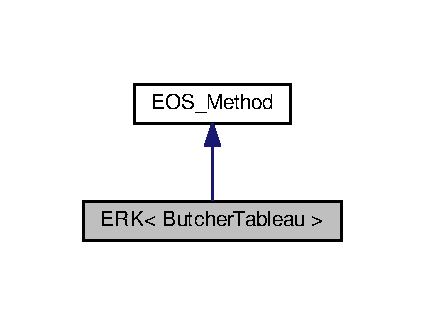
\includegraphics[width=204pt]{classERK__inherit__graph}
\end{center}
\end{figure}


Collaboration diagram for E\+RK$<$ Butcher\+Tableau $>$\+:\nopagebreak
\begin{figure}[H]
\begin{center}
\leavevmode
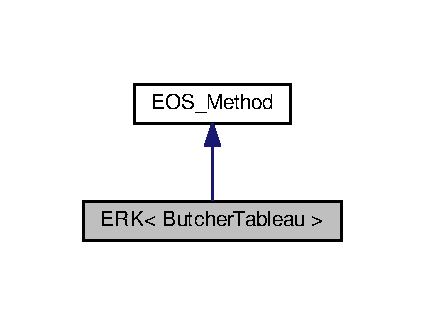
\includegraphics[width=204pt]{classERK__coll__graph}
\end{center}
\end{figure}
\subsection*{Public Member Functions}
\begin{DoxyCompactItemize}
\item 
\mbox{\Hypertarget{classERK_a2e9bccb7699bc97bd3800c25d86ee814}\label{classERK_a2e9bccb7699bc97bd3800c25d86ee814}} 
{\bfseries E\+RK} (\hyperlink{classTimeFunctor}{Time\+Functor} \&f, F\+P\+\_\+\+Type t0, dealii\+::\+Vector$<$ F\+P\+\_\+\+Type $>$ u0)
\item 
\mbox{\Hypertarget{classERK_afebd211b4d191591950da1544a1e2051}\label{classERK_afebd211b4d191591950da1544a1e2051}} 
dealii\+::\+Vector$<$ F\+P\+\_\+\+Type $>$ {\bfseries k\+\_\+increment} (F\+P\+\_\+\+Type t, const dealii\+::\+Vector$<$ F\+P\+\_\+\+Type $>$ \&u, F\+P\+\_\+\+Type h, const dealii\+::\+Vector$<$ F\+P\+\_\+\+Type $>$ \&b)
\item 
\mbox{\Hypertarget{classERK_a44ab542f5f577a322819c0a05a791db0}\label{classERK_a44ab542f5f577a322819c0a05a791db0}} 
std\+::pair$<$ dealii\+::\+Vector$<$ F\+P\+\_\+\+Type $>$, dealii\+::\+Full\+Matrix$<$ F\+P\+\_\+\+Type $>$ $>$ {\bfseries k\+\_\+variational} (F\+P\+\_\+\+Type t, const dealii\+::\+Vector$<$ F\+P\+\_\+\+Type $>$ \&u, F\+P\+\_\+\+Type h, const dealii\+::\+Vector$<$ F\+P\+\_\+\+Type $>$ \&b, const dealii\+::\+Full\+Matrix$<$ F\+P\+\_\+\+Type $>$ \&Y, \hyperlink{classTimeDivFunctor}{Time\+Div\+Functor} $\ast$F)
\item 
\mbox{\Hypertarget{classERK_ad6b4a1f225469f47dad5b17bb6791f30}\label{classERK_ad6b4a1f225469f47dad5b17bb6791f30}} 
virtual dealii\+::\+Vector$<$ F\+P\+\_\+\+Type $>$ {\bfseries increment\+\_\+function} (F\+P\+\_\+\+Type t, const dealii\+::\+Vector$<$ F\+P\+\_\+\+Type $>$ \&u, F\+P\+\_\+\+Type h) override
\item 
\mbox{\Hypertarget{classERK_ae3f71b3f5364ffcab63a715d95adb911}\label{classERK_ae3f71b3f5364ffcab63a715d95adb911}} 
size\+\_\+t {\bfseries n\+\_\+misfires} () const
\item 
\mbox{\Hypertarget{classERK_ac8835e6d68d903c7111da0b077821e3b}\label{classERK_ac8835e6d68d903c7111da0b077821e3b}} 
dealii\+::\+Full\+Matrix$<$ F\+P\+\_\+\+Type $>$ {\bfseries fund\+\_\+matrix} () const
\item 
\mbox{\Hypertarget{classERK_a7d23b9eb9d2f8defa0ca371e2f8cc2bc}\label{classERK_a7d23b9eb9d2f8defa0ca371e2f8cc2bc}} 
void {\bfseries iterate\+\_\+with\+\_\+ssc} (const F\+P\+\_\+\+Type t\+\_\+lim, const F\+P\+\_\+\+Type h0, const F\+P\+\_\+\+Type T\+OL, bool fundamental\+\_\+matrix)
\item 
\mbox{\Hypertarget{classERK_a6057b70fbd97bbe2e5b2d0233aef46a4}\label{classERK_a6057b70fbd97bbe2e5b2d0233aef46a4}} 
void {\bfseries print\+\_\+step\+\_\+size} (std\+::ostream \&out)
\end{DoxyCompactItemize}


The documentation for this class was generated from the following file\+:\begin{DoxyCompactItemize}
\item 
ivp/runge\+\_\+kutta.\+h\end{DoxyCompactItemize}

\hypertarget{structERK__04}{}\section{E\+R\+K\+\_\+04 Struct Reference}
\label{structERK__04}\index{E\+R\+K\+\_\+04@{E\+R\+K\+\_\+04}}


Collaboration diagram for E\+R\+K\+\_\+04\+:\nopagebreak
\begin{figure}[H]
\begin{center}
\leavevmode
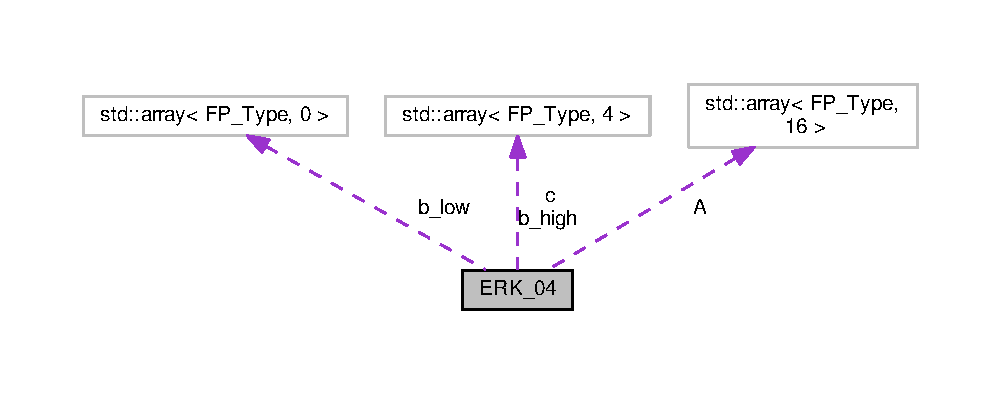
\includegraphics[width=350pt]{structERK__04__coll__graph}
\end{center}
\end{figure}
\subsection*{Public Attributes}
\begin{DoxyCompactItemize}
\item 
\mbox{\Hypertarget{structERK__04_ad51053d30094b589aad56694c40aa2e3}\label{structERK__04_ad51053d30094b589aad56694c40aa2e3}} 
const size\+\_\+t {\bfseries n} = 4
\item 
\mbox{\Hypertarget{structERK__04_a0eddad040c14f2cb43c398e3c7a3cdc3}\label{structERK__04_a0eddad040c14f2cb43c398e3c7a3cdc3}} 
const size\+\_\+t {\bfseries p} = 4
\item 
const std\+::array$<$ F\+P\+\_\+\+Type, 4 $>$ {\bfseries c}
\item 
const std\+::array$<$ F\+P\+\_\+\+Type, 16 $>$ {\bfseries A}
\item 
const std\+::array$<$ F\+P\+\_\+\+Type, 4 $>$ {\bfseries b\+\_\+high}
\item 
\mbox{\Hypertarget{structERK__04_a6f360ce6a229e0b3606a6d24f4469d5c}\label{structERK__04_a6f360ce6a229e0b3606a6d24f4469d5c}} 
const std\+::array$<$ F\+P\+\_\+\+Type, 0 $>$ {\bfseries b\+\_\+low} = \{\}
\end{DoxyCompactItemize}


\subsection{Member Data Documentation}
\mbox{\Hypertarget{structERK__04_a09c8913d7fa939adfdf8043561160a41}\label{structERK__04_a09c8913d7fa939adfdf8043561160a41}} 
\index{E\+R\+K\+\_\+04@{E\+R\+K\+\_\+04}!A@{A}}
\index{A@{A}!E\+R\+K\+\_\+04@{E\+R\+K\+\_\+04}}
\subsubsection{\texorpdfstring{A}{A}}
{\footnotesize\ttfamily const std\+::array$<$F\+P\+\_\+\+Type, 16$>$ E\+R\+K\+\_\+04\+::A}

{\bfseries Initial value\+:}
\begin{DoxyCode}
= \{
    0,    0,    0,    0,
    0.5,  0,    0,    0,
    0,    0.5,  0,    0,
    0,    0,    1.0,  0
  \}
\end{DoxyCode}
\mbox{\Hypertarget{structERK__04_a328bf104ac532f6c42164a9ef0d3b95c}\label{structERK__04_a328bf104ac532f6c42164a9ef0d3b95c}} 
\index{E\+R\+K\+\_\+04@{E\+R\+K\+\_\+04}!b\+\_\+high@{b\+\_\+high}}
\index{b\+\_\+high@{b\+\_\+high}!E\+R\+K\+\_\+04@{E\+R\+K\+\_\+04}}
\subsubsection{\texorpdfstring{b\+\_\+high}{b\_high}}
{\footnotesize\ttfamily const std\+::array$<$F\+P\+\_\+\+Type, 4$>$ E\+R\+K\+\_\+04\+::b\+\_\+high}

{\bfseries Initial value\+:}
\begin{DoxyCode}
= \{
    1./6, 2./6, 2./6, 1./6
  \}
\end{DoxyCode}
\mbox{\Hypertarget{structERK__04_a99fc8b005471e7b1946051149af63ea8}\label{structERK__04_a99fc8b005471e7b1946051149af63ea8}} 
\index{E\+R\+K\+\_\+04@{E\+R\+K\+\_\+04}!c@{c}}
\index{c@{c}!E\+R\+K\+\_\+04@{E\+R\+K\+\_\+04}}
\subsubsection{\texorpdfstring{c}{c}}
{\footnotesize\ttfamily const std\+::array$<$F\+P\+\_\+\+Type, 4$>$ E\+R\+K\+\_\+04\+::c}

{\bfseries Initial value\+:}
\begin{DoxyCode}
= \{
    0, 0.5, 0.5, 1.0
  \}
\end{DoxyCode}


The documentation for this struct was generated from the following file\+:\begin{DoxyCompactItemize}
\item 
ivp/tableau.\+h\end{DoxyCompactItemize}

\hypertarget{classERK__Test__O4}{}\section{E\+R\+K\+\_\+\+Test\+\_\+\+O4 Class Reference}
\label{classERK__Test__O4}\index{E\+R\+K\+\_\+\+Test\+\_\+\+O4@{E\+R\+K\+\_\+\+Test\+\_\+\+O4}}


Inheritance diagram for E\+R\+K\+\_\+\+Test\+\_\+\+O4\+:\nopagebreak
\begin{figure}[H]
\begin{center}
\leavevmode
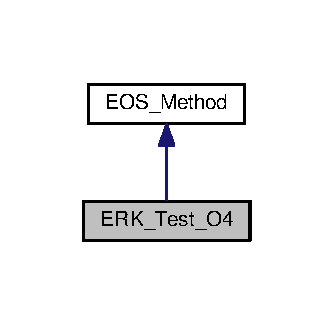
\includegraphics[width=160pt]{classERK__Test__O4__inherit__graph}
\end{center}
\end{figure}


Collaboration diagram for E\+R\+K\+\_\+\+Test\+\_\+\+O4\+:\nopagebreak
\begin{figure}[H]
\begin{center}
\leavevmode
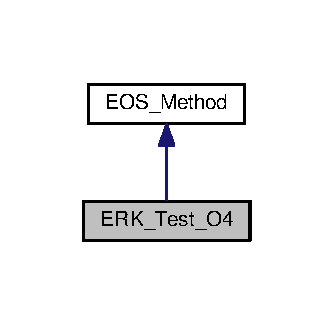
\includegraphics[width=160pt]{classERK__Test__O4__coll__graph}
\end{center}
\end{figure}
\subsection*{Public Member Functions}
\begin{DoxyCompactItemize}
\item 
\mbox{\Hypertarget{classERK__Test__O4_ad3bd6607faff8d74ff6759ac9963d0a4}\label{classERK__Test__O4_ad3bd6607faff8d74ff6759ac9963d0a4}} 
virtual dealii\+::\+Vector$<$ F\+P\+\_\+\+Type $>$ {\bfseries increment\+\_\+function} (F\+P\+\_\+\+Type t, const dealii\+::\+Vector$<$ F\+P\+\_\+\+Type $>$ \&u, F\+P\+\_\+\+Type h, t\+Vec\+Field \&f) override
\end{DoxyCompactItemize}


The documentation for this class was generated from the following file\+:\begin{DoxyCompactItemize}
\item 
test/test\+\_\+runge\+\_\+kutta.\+h\end{DoxyCompactItemize}

\hypertarget{classEuler}{}\section{Euler Class Reference}
\label{classEuler}\index{Euler@{Euler}}


Inheritance diagram for Euler\+:\nopagebreak
\begin{figure}[H]
\begin{center}
\leavevmode
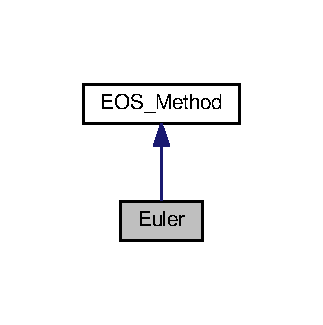
\includegraphics[width=167pt]{classEuler__inherit__graph}
\end{center}
\end{figure}


Collaboration diagram for Euler\+:\nopagebreak
\begin{figure}[H]
\begin{center}
\leavevmode
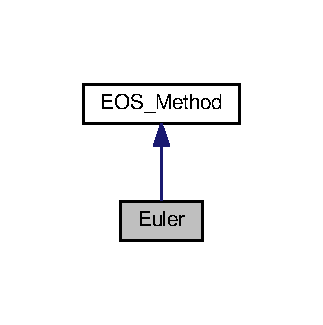
\includegraphics[width=167pt]{classEuler__coll__graph}
\end{center}
\end{figure}
\subsection*{Additional Inherited Members}


The documentation for this class was generated from the following file\+:\begin{DoxyCompactItemize}
\item 
ivp/euler.\+h\end{DoxyCompactItemize}

\hypertarget{classFAD__cWrapper}{}\section{F\+A\+D\+\_\+c\+Wrapper$<$ Callable $>$ Class Template Reference}
\label{classFAD__cWrapper}\index{F\+A\+D\+\_\+c\+Wrapper$<$ Callable $>$@{F\+A\+D\+\_\+c\+Wrapper$<$ Callable $>$}}


Inheritance diagram for F\+A\+D\+\_\+c\+Wrapper$<$ Callable $>$\+:\nopagebreak
\begin{figure}[H]
\begin{center}
\leavevmode
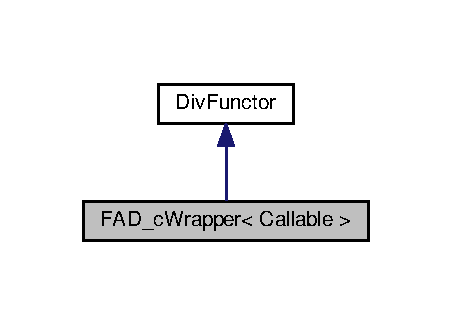
\includegraphics[width=217pt]{classFAD__cWrapper__inherit__graph}
\end{center}
\end{figure}


Collaboration diagram for F\+A\+D\+\_\+c\+Wrapper$<$ Callable $>$\+:\nopagebreak
\begin{figure}[H]
\begin{center}
\leavevmode
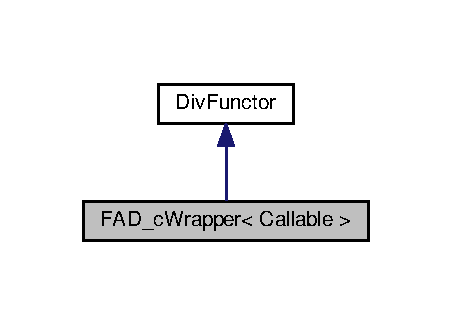
\includegraphics[width=217pt]{classFAD__cWrapper__coll__graph}
\end{center}
\end{figure}
\subsection*{Public Member Functions}
\begin{DoxyCompactItemize}
\item 
\mbox{\Hypertarget{classFAD__cWrapper_a4f9073b7ba4faa9624d2950960d9400d}\label{classFAD__cWrapper_a4f9073b7ba4faa9624d2950960d9400d}} 
{\bfseries F\+A\+D\+\_\+c\+Wrapper} (Callable \+\_\+f, size\+\_\+t \+\_\+dim)
\item 
\mbox{\Hypertarget{classFAD__cWrapper_a63579e11de4e55de607a84619ced86e2}\label{classFAD__cWrapper_a63579e11de4e55de607a84619ced86e2}} 
void {\bfseries init} (const dealii\+::\+Vector$<$ F\+P\+\_\+\+Type $>$ \&u)
\item 
\mbox{\Hypertarget{classFAD__cWrapper_a3f09fcd9fdb951eae4605cc3f57552cf}\label{classFAD__cWrapper_a3f09fcd9fdb951eae4605cc3f57552cf}} 
dealii\+::\+Vector$<$ F\+P\+\_\+\+Type $>$ {\bfseries value} () const
\item 
\mbox{\Hypertarget{classFAD__cWrapper_a6b167bc4c72bfea7c8690e61c9099652}\label{classFAD__cWrapper_a6b167bc4c72bfea7c8690e61c9099652}} 
virtual dealii\+::\+Vector$<$ F\+P\+\_\+\+Type $>$ {\bfseries operator()} (const dealii\+::\+Vector$<$ F\+P\+\_\+\+Type $>$ \&u) override
\item 
\mbox{\Hypertarget{classFAD__cWrapper_a21ebd0df0ef04881cc2c8f6a45df9a67}\label{classFAD__cWrapper_a21ebd0df0ef04881cc2c8f6a45df9a67}} 
dealii\+::\+Full\+Matrix$<$ F\+P\+\_\+\+Type $>$ {\bfseries diff} () const
\item 
\mbox{\Hypertarget{classFAD__cWrapper_add022de660756689b756924d5319c9ba}\label{classFAD__cWrapper_add022de660756689b756924d5319c9ba}} 
virtual dealii\+::\+Full\+Matrix$<$ F\+P\+\_\+\+Type $>$ {\bfseries diff} (const dealii\+::\+Vector$<$ F\+P\+\_\+\+Type $>$ \&u) override
\end{DoxyCompactItemize}


The documentation for this class was generated from the following file\+:\begin{DoxyCompactItemize}
\item 
base/forward\+\_\+ad.\+h\end{DoxyCompactItemize}

\hypertarget{classFAD__tWrapper}{}\section{F\+A\+D\+\_\+t\+Wrapper$<$ Callable $>$ Class Template Reference}
\label{classFAD__tWrapper}\index{F\+A\+D\+\_\+t\+Wrapper$<$ Callable $>$@{F\+A\+D\+\_\+t\+Wrapper$<$ Callable $>$}}


Inheritance diagram for F\+A\+D\+\_\+t\+Wrapper$<$ Callable $>$\+:\nopagebreak
\begin{figure}[H]
\begin{center}
\leavevmode
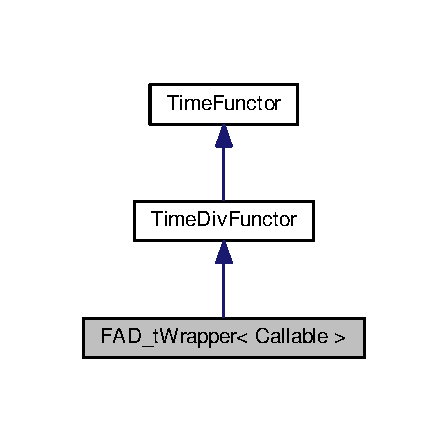
\includegraphics[width=215pt]{classFAD__tWrapper__inherit__graph}
\end{center}
\end{figure}


Collaboration diagram for F\+A\+D\+\_\+t\+Wrapper$<$ Callable $>$\+:\nopagebreak
\begin{figure}[H]
\begin{center}
\leavevmode
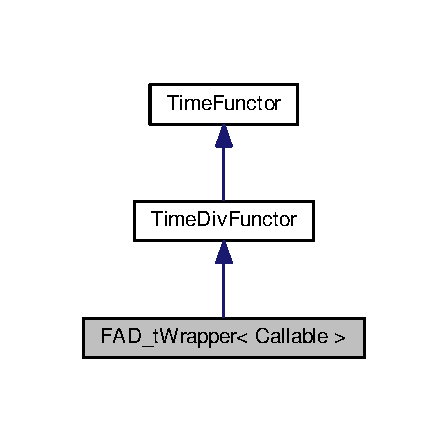
\includegraphics[width=215pt]{classFAD__tWrapper__coll__graph}
\end{center}
\end{figure}
\subsection*{Public Member Functions}
\begin{DoxyCompactItemize}
\item 
\mbox{\Hypertarget{classFAD__tWrapper_adf109515e54d838f27bc1f523331ac25}\label{classFAD__tWrapper_adf109515e54d838f27bc1f523331ac25}} 
{\bfseries F\+A\+D\+\_\+t\+Wrapper} (Callable f, size\+\_\+t dim)
\item 
\mbox{\Hypertarget{classFAD__tWrapper_ad0b635d7fc6f214d870ae4d03762612e}\label{classFAD__tWrapper_ad0b635d7fc6f214d870ae4d03762612e}} 
virtual Vector\+D2 {\bfseries operator()} (F\+P\+\_\+\+Type t, const Vector\+D2 \&u) override
\item 
\mbox{\Hypertarget{classFAD__tWrapper_aca8b9ccaf25becd93620776d404f20d8}\label{classFAD__tWrapper_aca8b9ccaf25becd93620776d404f20d8}} 
virtual Matrix\+D2 {\bfseries diff} (F\+P\+\_\+\+Type t, const Vector\+D2 \&u) override
\end{DoxyCompactItemize}


The documentation for this class was generated from the following file\+:\begin{DoxyCompactItemize}
\item 
base/forward\+\_\+ad.\+h\end{DoxyCompactItemize}

\hypertarget{structKARP}{}\section{K\+A\+RP Struct Reference}
\label{structKARP}\index{K\+A\+RP@{K\+A\+RP}}


Butcher Tableau for the Cash-\/\+Karp method of order 5(4).  




{\ttfamily \#include $<$tableau.\+h$>$}



Collaboration diagram for K\+A\+RP\+:\nopagebreak
\begin{figure}[H]
\begin{center}
\leavevmode
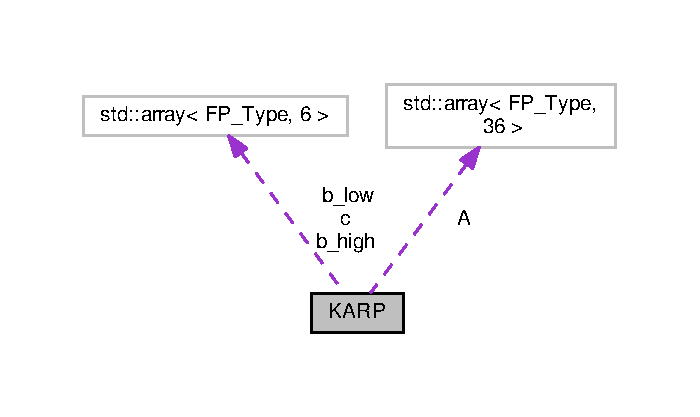
\includegraphics[width=336pt]{structKARP__coll__graph}
\end{center}
\end{figure}
\subsection*{Public Attributes}
\begin{DoxyCompactItemize}
\item 
\mbox{\Hypertarget{structKARP_ae4748bfe9d63b1aaa28a8ea47072f8e3}\label{structKARP_ae4748bfe9d63b1aaa28a8ea47072f8e3}} 
const size\+\_\+t {\bfseries n} = 6
\item 
\mbox{\Hypertarget{structKARP_a68a9bee99c22bab5ba56a392e2fa6cb0}\label{structKARP_a68a9bee99c22bab5ba56a392e2fa6cb0}} 
const size\+\_\+t {\bfseries p} = 4
\item 
const std\+::array$<$ F\+P\+\_\+\+Type, 6 $>$ {\bfseries c}
\item 
const std\+::array$<$ F\+P\+\_\+\+Type, 36 $>$ {\bfseries A}
\item 
const std\+::array$<$ F\+P\+\_\+\+Type, 6 $>$ {\bfseries b\+\_\+high}
\item 
const std\+::array$<$ F\+P\+\_\+\+Type, 6 $>$ {\bfseries b\+\_\+low}
\end{DoxyCompactItemize}


\subsection{Detailed Description}
Butcher Tableau for the Cash-\/\+Karp method of order 5(4). 

Ddetails on this method and its lower order variants are available in the original paper\+:

\href{http://www.elegio.it/mc2/rk/doc/p201-cash-karp.pdf}{\tt http\+://www.\+elegio.\+it/mc2/rk/doc/p201-\/cash-\/karp.\+pdf} 

\subsection{Member Data Documentation}
\mbox{\Hypertarget{structKARP_a5e62cee865e772c7a7e7072f578c658d}\label{structKARP_a5e62cee865e772c7a7e7072f578c658d}} 
\index{K\+A\+RP@{K\+A\+RP}!A@{A}}
\index{A@{A}!K\+A\+RP@{K\+A\+RP}}
\subsubsection{\texorpdfstring{A}{A}}
{\footnotesize\ttfamily const std\+::array$<$F\+P\+\_\+\+Type, 36$>$ K\+A\+R\+P\+::A}

{\bfseries Initial value\+:}
\begin{DoxyCode}
= \{
    0,            0,         0,           0,              0,          0,
    1./5,         0,         0,           0,              0,          0,
    3./40,        9./40,     0,           0,              0,          0,
    3./10,        -9./10,    6./5,        0,              0,          0,
    -11./54,      5./2,      -70./27,     35./27,         0,          0,
    1631./55296,  175./512,  575./13824,  44275./110592,  253./4096,  0
  \}
\end{DoxyCode}
\mbox{\Hypertarget{structKARP_af682eefba6a62bb8bf72efc293e2e361}\label{structKARP_af682eefba6a62bb8bf72efc293e2e361}} 
\index{K\+A\+RP@{K\+A\+RP}!b\+\_\+high@{b\+\_\+high}}
\index{b\+\_\+high@{b\+\_\+high}!K\+A\+RP@{K\+A\+RP}}
\subsubsection{\texorpdfstring{b\+\_\+high}{b\_high}}
{\footnotesize\ttfamily const std\+::array$<$F\+P\+\_\+\+Type, 6$>$ K\+A\+R\+P\+::b\+\_\+high}

{\bfseries Initial value\+:}
\begin{DoxyCode}
= \{
    37./378, 0, 250./621, 125./594, 0, 512./1771
  \}
\end{DoxyCode}
\mbox{\Hypertarget{structKARP_a2833bea5896058e8ad8256a41e4e04d2}\label{structKARP_a2833bea5896058e8ad8256a41e4e04d2}} 
\index{K\+A\+RP@{K\+A\+RP}!b\+\_\+low@{b\+\_\+low}}
\index{b\+\_\+low@{b\+\_\+low}!K\+A\+RP@{K\+A\+RP}}
\subsubsection{\texorpdfstring{b\+\_\+low}{b\_low}}
{\footnotesize\ttfamily const std\+::array$<$F\+P\+\_\+\+Type, 6$>$ K\+A\+R\+P\+::b\+\_\+low}

{\bfseries Initial value\+:}
\begin{DoxyCode}
= \{
    2825./27648, 0, 18575./48384, 13525./55296, 277./14336, 1./4
  \}
\end{DoxyCode}
\mbox{\Hypertarget{structKARP_a1b174009b3b9f53824e6d59fc92cb56d}\label{structKARP_a1b174009b3b9f53824e6d59fc92cb56d}} 
\index{K\+A\+RP@{K\+A\+RP}!c@{c}}
\index{c@{c}!K\+A\+RP@{K\+A\+RP}}
\subsubsection{\texorpdfstring{c}{c}}
{\footnotesize\ttfamily const std\+::array$<$F\+P\+\_\+\+Type, 6$>$ K\+A\+R\+P\+::c}

{\bfseries Initial value\+:}
\begin{DoxyCode}
= \{
    0, 1./5, 3./10, 3./5, 1, 7./8
  \}
\end{DoxyCode}


The documentation for this struct was generated from the following file\+:\begin{DoxyCompactItemize}
\item 
ivp/tableau.\+h\end{DoxyCompactItemize}

\hypertarget{classNewton}{}\section{Newton$<$ Callable $>$ Class Template Reference}
\label{classNewton}\index{Newton$<$ Callable $>$@{Newton$<$ Callable $>$}}
\subsection*{Public Member Functions}
\begin{DoxyCompactItemize}
\item 
\mbox{\Hypertarget{classNewton_ae4ba28e81968382bfdd3213bbc762611}\label{classNewton_ae4ba28e81968382bfdd3213bbc762611}} 
{\bfseries Newton} (Callable \+\_\+f, size\+\_\+t \+\_\+dim)
\item 
\mbox{\Hypertarget{classNewton_a2e7db9daefa5fb97a77de03cadd132e4}\label{classNewton_a2e7db9daefa5fb97a77de03cadd132e4}} 
dealii\+::\+Vector$<$ F\+P\+\_\+\+Type $>$ {\bfseries step} (const dealii\+::\+Full\+Matrix$<$ F\+P\+\_\+\+Type $>$ \&J, const dealii\+::\+Vector$<$ F\+P\+\_\+\+Type $>$ \&x, bool step\+\_\+size\+\_\+control=true, size\+\_\+t ssc\+\_\+limit=20)
\item 
\mbox{\Hypertarget{classNewton_ab3fde95489168338724e34d35a17d58d}\label{classNewton_ab3fde95489168338724e34d35a17d58d}} 
bool {\bfseries stopping\+\_\+criterion} (F\+P\+\_\+\+Type T\+OL) const
\item 
\mbox{\Hypertarget{classNewton_a7914b92f40c22ddc30926657663c386d}\label{classNewton_a7914b92f40c22ddc30926657663c386d}} 
dealii\+::\+Vector$<$ F\+P\+\_\+\+Type $>$ {\bfseries iterate} (dealii\+::\+Vector$<$ F\+P\+\_\+\+Type $>$ s, size\+\_\+t step\+\_\+limit=50)
\end{DoxyCompactItemize}


The documentation for this class was generated from the following file\+:\begin{DoxyCompactItemize}
\item 
algo/newton.\+h\end{DoxyCompactItemize}

\hypertarget{classSF__Automatic}{}\section{S\+F\+\_\+\+Automatic$<$ M, M\+\_\+\+Var $>$ Class Template Reference}
\label{classSF__Automatic}\index{S\+F\+\_\+\+Automatic$<$ M, M\+\_\+\+Var $>$@{S\+F\+\_\+\+Automatic$<$ M, M\+\_\+\+Var $>$}}


Inheritance diagram for S\+F\+\_\+\+Automatic$<$ M, M\+\_\+\+Var $>$\+:\nopagebreak
\begin{figure}[H]
\begin{center}
\leavevmode
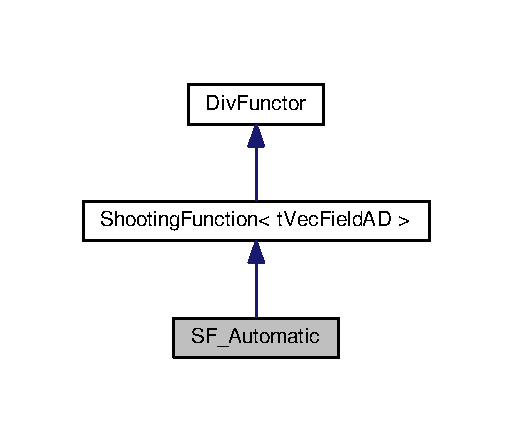
\includegraphics[width=190pt]{classSF__Automatic__inherit__graph}
\end{center}
\end{figure}


Collaboration diagram for S\+F\+\_\+\+Automatic$<$ M, M\+\_\+\+Var $>$\+:\nopagebreak
\begin{figure}[H]
\begin{center}
\leavevmode
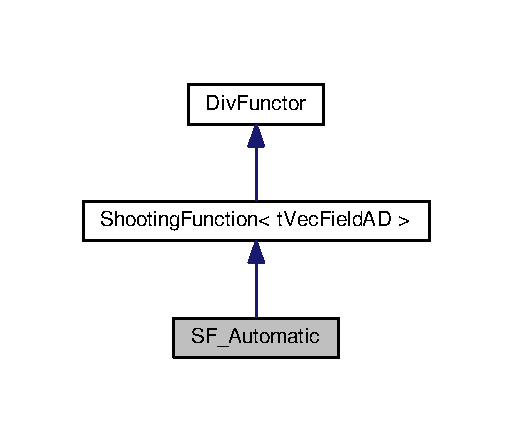
\includegraphics[width=190pt]{classSF__Automatic__coll__graph}
\end{center}
\end{figure}
\subsection*{Public Member Functions}
\begin{DoxyCompactItemize}
\item 
\mbox{\Hypertarget{classSF__Automatic_a1805f867ada14ddc960d72da0c8717c5}\label{classSF__Automatic_a1805f867ada14ddc960d72da0c8717c5}} 
virtual Vector\+D2 {\bfseries solve\+\_\+y} (F\+P\+\_\+\+Type t0, F\+P\+\_\+\+Type t1, const Vector\+D2 \&s) override
\item 
\mbox{\Hypertarget{classSF__Automatic_a42df8fe14e093057d2fe40cb42a0460e}\label{classSF__Automatic_a42df8fe14e093057d2fe40cb42a0460e}} 
virtual std\+::pair$<$ Vector\+D2, Matrix\+D2 $>$ {\bfseries solve\+\_\+Z} (F\+P\+\_\+\+Type t0, F\+P\+\_\+\+Type t1, const Vector\+D2 \&s) override
\end{DoxyCompactItemize}


The documentation for this class was generated from the following file\+:\begin{DoxyCompactItemize}
\item 
bvp/shooting.\+h\end{DoxyCompactItemize}

\hypertarget{classSF__External}{}\section{S\+F\+\_\+\+External$<$ M $>$ Class Template Reference}
\label{classSF__External}\index{S\+F\+\_\+\+External$<$ M $>$@{S\+F\+\_\+\+External$<$ M $>$}}


Inheritance diagram for S\+F\+\_\+\+External$<$ M $>$\+:\nopagebreak
\begin{figure}[H]
\begin{center}
\leavevmode
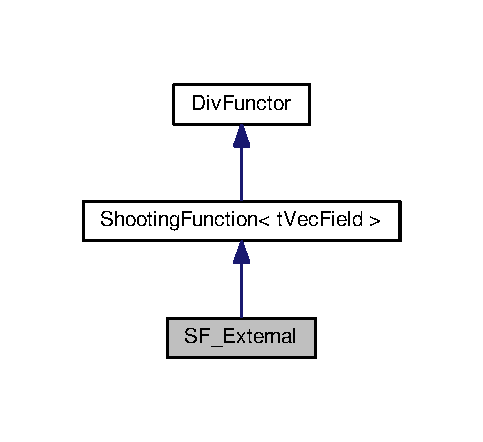
\includegraphics[width=177pt]{classSF__External__inherit__graph}
\end{center}
\end{figure}


Collaboration diagram for S\+F\+\_\+\+External$<$ M $>$\+:\nopagebreak
\begin{figure}[H]
\begin{center}
\leavevmode
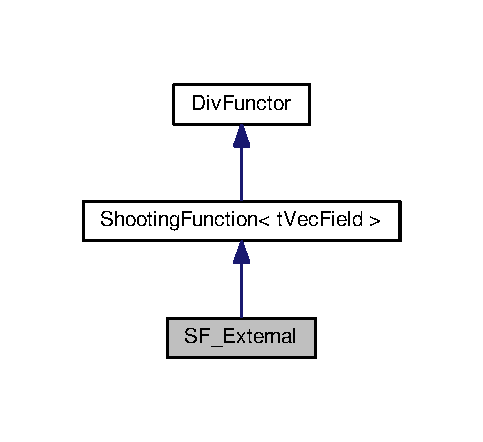
\includegraphics[width=177pt]{classSF__External__coll__graph}
\end{center}
\end{figure}
\subsection*{Public Member Functions}
\begin{DoxyCompactItemize}
\item 
\mbox{\Hypertarget{classSF__External_a4c59ab31f0bb2ab9663b5137655a6266}\label{classSF__External_a4c59ab31f0bb2ab9663b5137655a6266}} 
virtual Vector\+D2 \hyperlink{classSF__External_a4c59ab31f0bb2ab9663b5137655a6266}{solve\+\_\+y} (F\+P\+\_\+\+Type t0, F\+P\+\_\+\+Type t1, const Vector\+D2 \&s) override
\begin{DoxyCompactList}\small\item\em Solve $y(t; t_0, s)$ in $t = t_1$. \end{DoxyCompactList}\item 
virtual std\+::pair$<$ Vector\+D2, Matrix\+D2 $>$ \hyperlink{classSF__External_a72c762001bc0a4bc43ac82aba45ad3ba}{solve\+\_\+Z} (F\+P\+\_\+\+Type t0, F\+P\+\_\+\+Type t1, const Vector\+D2 \&s) override
\begin{DoxyCompactList}\small\item\em Solve $D_s y(t; t_0, s)$ in $t = t_1$ by external differentation. \end{DoxyCompactList}\end{DoxyCompactItemize}


\subsection{Member Function Documentation}
\mbox{\Hypertarget{classSF__External_a72c762001bc0a4bc43ac82aba45ad3ba}\label{classSF__External_a72c762001bc0a4bc43ac82aba45ad3ba}} 
\index{S\+F\+\_\+\+External@{S\+F\+\_\+\+External}!solve\+\_\+Z@{solve\+\_\+Z}}
\index{solve\+\_\+Z@{solve\+\_\+Z}!S\+F\+\_\+\+External@{S\+F\+\_\+\+External}}
\subsubsection{\texorpdfstring{solve\+\_\+\+Z()}{solve\_Z()}}
{\footnotesize\ttfamily template$<$typename M $>$ \\
virtual std\+::pair$<$Vector\+D2, Matrix\+D2$>$ \hyperlink{classSF__External}{S\+F\+\_\+\+External}$<$ M $>$\+::solve\+\_\+Z (\begin{DoxyParamCaption}\item[{F\+P\+\_\+\+Type}]{t0,  }\item[{F\+P\+\_\+\+Type}]{t1,  }\item[{const Vector\+D2 \&}]{s }\end{DoxyParamCaption})\hspace{0.3cm}{\ttfamily [inline]}, {\ttfamily [override]}, {\ttfamily [virtual]}}



Solve $D_s y(t; t_0, s)$ in $t = t_1$ by external differentation. 

For the choice of $TOL$ in the adaptive method and the constant $eps$, see Stoer, Num. Math. 2, pp. 192. 

Implements \hyperlink{classShootingFunction_a41360056996ee70c43c4538acd6e28d8}{Shooting\+Function}.



The documentation for this class was generated from the following file\+:\begin{DoxyCompactItemize}
\item 
bvp/shooting.\+h\end{DoxyCompactItemize}

\hypertarget{classShootingFunction}{}\section{Shooting\+Function Class Reference}
\label{classShootingFunction}\index{Shooting\+Function@{Shooting\+Function}}


Inheritance diagram for Shooting\+Function\+:
\nopagebreak
\begin{figure}[H]
\begin{center}
\leavevmode
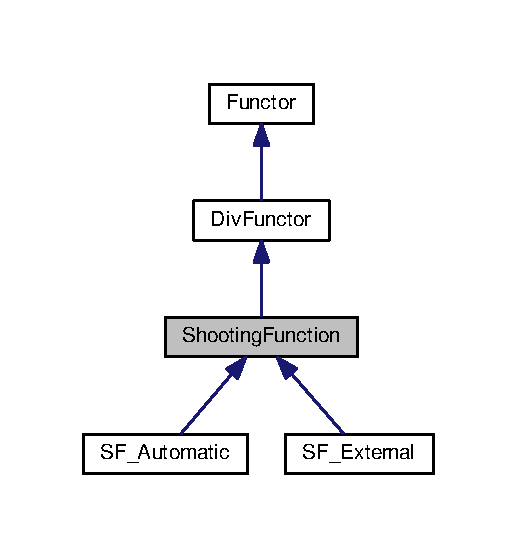
\includegraphics[width=248pt]{classShootingFunction__inherit__graph}
\end{center}
\end{figure}
\subsection*{Public Member Functions}
\begin{DoxyCompactItemize}
\item 
\mbox{\Hypertarget{classShootingFunction_a9621110f76332ab774b15b7574a43c16}\label{classShootingFunction_a9621110f76332ab774b15b7574a43c16}} 
{\bfseries Shooting\+Function} (\hyperlink{classTimeFunctor}{Time\+Functor} \&\+\_\+f)
\item 
\mbox{\Hypertarget{classShootingFunction_a2fff86465b3e0ee1e4e29d8691dbd8f5}\label{classShootingFunction_a2fff86465b3e0ee1e4e29d8691dbd8f5}} 
virtual dealii\+::\+Vector$<$ F\+P\+\_\+\+Type $>$ {\bfseries solve\+\_\+y} (F\+P\+\_\+\+Type t0, F\+P\+\_\+\+Type t1, const dealii\+::\+Vector$<$ F\+P\+\_\+\+Type $>$ \&s)=0
\item 
\mbox{\Hypertarget{classShootingFunction_a679b8e1483215ced4212dd7acb0001f8}\label{classShootingFunction_a679b8e1483215ced4212dd7acb0001f8}} 
virtual dealii\+::\+Full\+Matrix$<$ F\+P\+\_\+\+Type $>$ {\bfseries solve\+\_\+Z} (F\+P\+\_\+\+Type t0, F\+P\+\_\+\+Type t1, const dealii\+::\+Vector$<$ F\+P\+\_\+\+Type $>$ \&s)=0
\end{DoxyCompactItemize}
\subsection*{Friends}
\begin{DoxyCompactItemize}
\item 
\mbox{\Hypertarget{classShootingFunction_a93dbf39ac4cbbc98d7d42b86d98179eb}\label{classShootingFunction_a93dbf39ac4cbbc98d7d42b86d98179eb}} 
class {\bfseries S\+F\+\_\+\+External}
\item 
\mbox{\Hypertarget{classShootingFunction_ab9857bb910ee9206e4888bdc358f0ecb}\label{classShootingFunction_ab9857bb910ee9206e4888bdc358f0ecb}} 
class {\bfseries S\+F\+\_\+\+Automatic}
\item 
\mbox{\Hypertarget{classShootingFunction_acf7e9fe888f96c8f5b3243c0848c0fcd}\label{classShootingFunction_acf7e9fe888f96c8f5b3243c0848c0fcd}} 
class {\bfseries S\+F\+\_\+\+Manual}
\end{DoxyCompactItemize}


The documentation for this class was generated from the following file\+:\begin{DoxyCompactItemize}
\item 
bvp/shooting.\+h\end{DoxyCompactItemize}

\hypertarget{classSimpleBVP}{}\section{Simple\+B\+VP$<$ Diff\+Method $>$ Class Template Reference}
\label{classSimpleBVP}\index{Simple\+B\+V\+P$<$ Diff\+Method $>$@{Simple\+B\+V\+P$<$ Diff\+Method $>$}}
\subsection*{Public Member Functions}
\begin{DoxyCompactItemize}
\item 
\mbox{\Hypertarget{classSimpleBVP_a4e0d2aec5b55b5bb68938361d58459cc}\label{classSimpleBVP_a4e0d2aec5b55b5bb68938361d58459cc}} 
{\bfseries Simple\+B\+VP} (\hyperlink{classTimeFunctor}{Time\+Functor} \&\+\_\+f, F\+P\+\_\+\+Type \+\_\+a, F\+P\+\_\+\+Type \+\_\+b, dealii\+::\+Vector$<$ F\+P\+\_\+\+Type $>$ \+\_\+c)
\item 
\mbox{\Hypertarget{classSimpleBVP_a7a82615c678f4f57648788b2d788d32e}\label{classSimpleBVP_a7a82615c678f4f57648788b2d788d32e}} 
void {\bfseries single\+\_\+shooting} (const std\+::vector$<$ dealii\+::\+Vector$<$ F\+P\+\_\+\+Type $>$ $>$ \&start)
\item 
\mbox{\Hypertarget{classSimpleBVP_a36f55e9851a3858cf8133ec8391527fc}\label{classSimpleBVP_a36f55e9851a3858cf8133ec8391527fc}} 
void {\bfseries shooting\+\_\+graph} (size\+\_\+t dim, const std\+::vector$<$ dealii\+::\+Vector$<$ F\+P\+\_\+\+Type $>$ $>$ \&range, std\+::ofstream \&output\+\_\+file)
\end{DoxyCompactItemize}


The documentation for this class was generated from the following file\+:\begin{DoxyCompactItemize}
\item 
bvp/linear.\+h\end{DoxyCompactItemize}

\hypertarget{classTimeDivFunctor}{}\section{Time\+Div\+Functor Class Reference}
\label{classTimeDivFunctor}\index{Time\+Div\+Functor@{Time\+Div\+Functor}}


Inheritance diagram for Time\+Div\+Functor\+:
\nopagebreak
\begin{figure}[H]
\begin{center}
\leavevmode
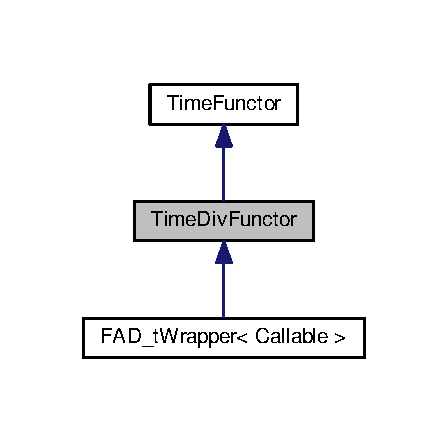
\includegraphics[width=215pt]{classTimeDivFunctor__inherit__graph}
\end{center}
\end{figure}


Collaboration diagram for Time\+Div\+Functor\+:
\nopagebreak
\begin{figure}[H]
\begin{center}
\leavevmode
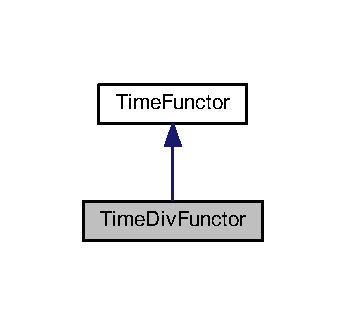
\includegraphics[width=166pt]{classTimeDivFunctor__coll__graph}
\end{center}
\end{figure}
\subsection*{Public Member Functions}
\begin{DoxyCompactItemize}
\item 
\mbox{\Hypertarget{classTimeDivFunctor_acbdba504a35a59e0b6687718b9d7d8ff}\label{classTimeDivFunctor_acbdba504a35a59e0b6687718b9d7d8ff}} 
virtual Matrix\+D2 {\bfseries diff} (F\+P\+\_\+\+Type t, const Vector\+D2 \&u)=0
\end{DoxyCompactItemize}


The documentation for this class was generated from the following file\+:\begin{DoxyCompactItemize}
\item 
lac/lac\+\_\+types.\+h\end{DoxyCompactItemize}

%--- End generated contents ---

% Index
\backmatter
\newpage
\phantomsection
\clearemptydoublepage
\addcontentsline{toc}{chapter}{Index}
\printindex

\end{document}
